% =============================================================================
%  KeyLoggd: presenter's companion
%  Every keyword on the slides, explained in plain language, in slide order.
%  Compile with XeLaTeX:   xelatex keyloggd-notes.tex   (twice, for the contents)
% =============================================================================
\documentclass[11pt,a4paper]{article}

\usepackage{fontspec}
\setsansfont{Inter}[
  Extension=.otf, UprightFont=*-Regular, BoldFont=*-SemiBold,
  ItalicFont=*-Italic, BoldItalicFont=*-SemiBoldItalic, Scale=0.95]
\setmainfont{Inter}[
  Extension=.otf, UprightFont=*-Regular, BoldFont=*-SemiBold,
  ItalicFont=*-Italic, BoldItalicFont=*-SemiBoldItalic, Scale=0.95]
\setmonofont{Consolas}[Scale=0.95]
\newfontfamily\titlefont{Georgia}[Ligatures=TeX]
\usepackage{amsmath}
\usepackage{unicode-math}
\setmathfont{Cambria Math}

\usepackage[a4paper,margin=2.2cm,top=2.4cm,bottom=2.4cm]{geometry}
\usepackage{xcolor}
\usepackage{fontawesome5}
\usepackage[most]{tcolorbox}
\usepackage{tikz}
\usetikzlibrary{arrows.meta,calc,decorations.pathreplacing}
\usepackage{booktabs,array,tabularx}
\usepackage[hidelinks]{hyperref}

\definecolor{ink}{HTML}{262624}
\definecolor{cream}{HTML}{F0EEE6}
\definecolor{terra}{HTML}{D97757}
\definecolor{terradk}{HTML}{B85F42}
\definecolor{sky}{HTML}{3987E5}
\definecolor{sage}{HTML}{5F9A68}
\definecolor{amber}{HTML}{D9A257}
\definecolor{rose}{HTML}{E0685A}
\definecolor{muted}{HTML}{8A8985}
\definecolor{line}{HTML}{E6E2D8}
\definecolor{soft}{HTML}{F5F3EE}

\setlength\parindent{0pt}
\setlength\parskip{4pt}
\linespread{1.12}

% section heading: number, title, short terracotta rule
\newcommand\bigsec[1]{%
  \par\vspace{18pt}\refstepcounter{section}%
  \addcontentsline{toc}{section}{\protect\numberline{\thesection}#1}%
  \noindent{\titlefont\LARGE\color{terra}\thesection\quad\color{ink}#1}\par\nopagebreak
  \vspace{2pt}\noindent{\color{terra}\rule{2.2cm}{1.4pt}}\par\nopagebreak\vspace{8pt}}

% ---- the building blocks --------------------------------------------------
% \slide{title of the slide it belongs to}
\newcommand\slide[1]{%
  \par\vspace{14pt}\addcontentsline{toc}{subsection}{#1}%
  \noindent{\titlefont\Large\color{ink}\textcolor{muted}{\normalsize\faDesktop}\enspace #1}\par\nopagebreak\vspace{3pt}}
% \term{keyword}{explanation}
\newcommand\term[2]{%
  \par\vspace{3pt}\noindent
  \begin{minipage}[t]{\linewidth}
    {\bfseries\color{terradk}#1}\par\vspace{1pt}
    #2
  \end{minipage}\par}
% \say{what to say on stage}
\newcommand\say[1]{\par\noindent{\color{sky}\small\faMicrophone\enspace\emph{On stage:} #1}\par}
\newtcolorbox{note}[1][]{enhanced, colback=soft, colframe=line, boxrule=0.6pt, arc=4pt,
  left=8pt, right=8pt, top=5pt, bottom=5pt, #1}
\newtcolorbox{keybox}[1]{enhanced, colback=white, colframe=terra!55, boxrule=0.7pt, arc=5pt,
  left=9pt, right=9pt, top=5pt, bottom=6pt, title={#1}, coltitle=terradk, colbacktitle=white,
  fonttitle=\bfseries, titlerule=0pt}

\begin{document}

% ---------------------------------------------------------------- cover ------
\begin{titlepage}
\begin{tikzpicture}[remember picture,overlay]
  \fill[ink] (current page.south west) rectangle (current page.north east);
  \foreach \d/\f [count=\i from 0] in {69/128,72/88,72/25,94/-31,103/49,55/113,97/39,96/50,
      70/266,79/2,125/-115,92/-9,112/80,87/82,54/300,72/57,78/89,55/201,110/-22,94/282} {
    \fill[terra] ($(current page.south west)+(2.2+\i*0.82,5)$) rectangle ++(0.32,\d*0.012);
    \fill[sky] ($(current page.south west)+(2.58+\i*0.82,5)$) rectangle ++(0.32,\f*0.009);
  }
  \node[anchor=north west,text=terra,font=\small\bfseries] at ($(current page.north west)+(2.2,-4)$)
    {\faKeyboard\enspace PRESENTER'S COMPANION};
  \node[anchor=north west,text=cream,font=\titlefont\fontsize{54}{58}\selectfont] at ($(current page.north west)+(2.1,-4.7)$) {KeyLoggd};
  \node[anchor=north west,text=cream!80,font=\Large,text width=15cm] at ($(current page.north west)+(2.2,-7.2)$)
    {Every keyword on the slides, explained in plain language, in the order you will present them.};
  \node[anchor=north west,text=muted,font=\normalsize,text width=15cm] at ($(current page.north west)+(2.2,-9.2)$)
    {Private notes. Blue \faMicrophone\ lines are suggested wording for the talk. The last pages hold the numbers to remember and the questions you are most likely to get.};
\end{tikzpicture}
\end{titlepage}

\tableofcontents
\newpage

% =============================================================================
\bigsec{How to use these notes}
% =============================================================================
The notes follow the slides in order. Each slide title appears as a heading, followed by the words on it that
need explaining. For each word you get:

\begin{itemize}
  \item a \textbf{plain explanation}: what it is, without jargon;
  \item where it helps, \textbf{why we use it} in KeyLoggd;
  \item for the important ones, a \textcolor{sky}{\faMicrophone\ \emph{On stage}} line you can say almost word for word.
\end{itemize}

\begin{note}
\textbf{The whole project in three sentences.} Everyone presses and releases keys with a personal rhythm. KeyLoggd records
that rhythm while you play a typing game, turns it into 26 numbers that describe \emph{how} you type, and stores an average
profile for you. Later, when someone types, it compares their numbers to every stored profile and names the closest one,
or says ``unrecognised'' if nobody is close enough.
\end{note}

\begin{center}
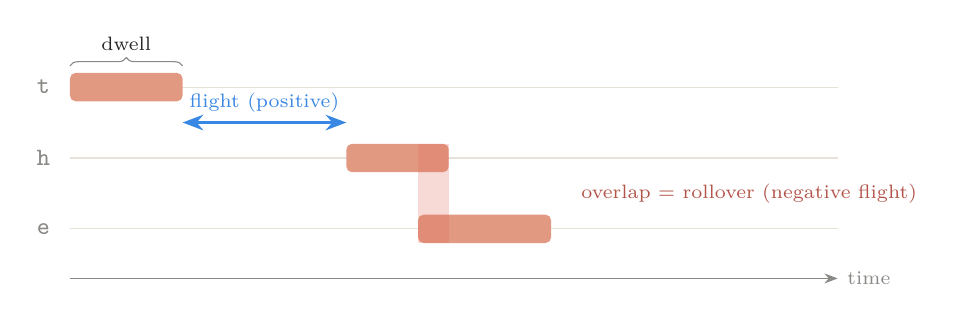
\begin{tikzpicture}[x=13cm,y=0.9cm]
  \foreach \k/\y in {t/2,h/1,e/0} {\node[anchor=east,font=\ttfamily\small,text=muted] at (-0.01,\y) {\k}; \draw[line] (0,\y) -- (0.75,\y);}
  \fill[terra!75,rounded corners=2pt] (0.00,1.8) rectangle (0.11,2.2);
  \fill[terra!75,rounded corners=2pt] (0.27,0.8) rectangle (0.37,1.2);
  \fill[terra!75,rounded corners=2pt] (0.34,-0.2) rectangle (0.47,0.2);
  \draw[decorate,decoration={brace,amplitude=3pt},muted] (0,2.3) -- (0.11,2.3) node[midway,above=2pt,font=\scriptsize,text=ink] {dwell};
  \draw[sky,line width=1pt,{Stealth}-{Stealth}] (0.11,1.5) -- (0.27,1.5) node[midway,above,font=\scriptsize,text=sky] {flight (positive)};
  \fill[rose,opacity=0.25] (0.34,-0.2) rectangle (0.37,1.2);
  \node[font=\scriptsize,text=rose!80!black,anchor=west] at (0.49,0.5) {overlap = rollover (negative flight)};
  \draw[muted,-{Stealth}] (0,-0.7) -- (0.75,-0.7) node[right,font=\scriptsize] {time};
\end{tikzpicture}
\end{center}
{\small\color{muted}The only two measurements everything is built from: how long each key is held (\textbf{dwell}), and the gap until
the next key goes down (\textbf{flight}).}

% =============================================================================
\bigsec{Why keystrokes?}
% =============================================================================

\slide{Title slide}
\term{Keystroke dynamics}{The study of \emph{how} someone types, not \emph{what} they type: the timing of each key press
and release. It is a kind of behavioural biometric.}
\term{Behavioural biometric}{A way of recognising a person from something they \emph{do} (typing, walking, signing, moving a mouse),
as opposed to a \emph{physiological} biometric, which uses something they physically \emph{are} (fingerprint, face, iris).}
\term{Rhythm}{Our informal word for the pattern of holds and gaps as you type. The bars on the title slide are a real
32-key sample from our data: orange = dwell, blue = flight.}
\term{Think-pause}{A long gap while the typist stops to think or read (1.37\,s in the title-slide sample). It is about 20 times a
normal gap, which is why the pipeline has to be careful with averages.}

\slide{Every login factor has a weak spot}
\term{Authentication}{Proving you are who you claim to be. Different from \emph{authorisation}, which decides what you are
allowed to do once you are in.}
\term{Authentication factor}{A category of proof. The classic three are something you \emph{know} (password), something you
\emph{have} (phone, token), and something you \emph{are} (fingerprint). Keystroke dynamics adds a fourth: something you \emph{do}.}
\term{PIN / pattern}{Short secrets, a number or a swipe shape. Same weaknesses as passwords, just shorter.}
\term{Phishing}{Tricking someone into typing their secret into a fake site or form.}
\term{Credential reuse}{Using the same password on many sites, so one leak unlocks all of them.}
\term{Shoulder-surfing}{Watching someone type their password or PIN.}
\term{Reset flow}{The ``forgot password'' process. It is often the weakest link, because it has to let you in without the password.}
\term{OTP (one-time password)}{A short code that works once, usually sent by SMS or generated by an app.}
\term{2FA (two-factor authentication)}{Requiring two different factors, typically password plus OTP.}
\term{SIM swap}{An attacker convinces a mobile carrier to move your number to their SIM card, so your SMS codes go to them.}
\term{Real-time phishing}{A fake site that forwards your OTP to the real site instantly, before it expires.}
\term{Sensor}{Dedicated hardware to read a biometric (fingerprint reader, depth camera). Keystroke dynamics needs none: the keyboard is the sensor.}
\term{Revocable / irrevocable}{Whether you can replace the secret after it leaks. You can change a password, but not your fingerprint.}
\term{Spoofing}{Faking a biometric: a printed photo for face unlock, a silicone mould of a fingerprint.}
\say{``Passwords get phished, phones get SIM-swapped, fingerprints need a sensor and can't be changed. And all three only check you once, at the door.''}

\slide{The one-time gate problem}
\term{Session}{The period after you log in, during which the system trusts you without asking again.}
\term{Session takeover}{Someone else using your already-open session, for example on a laptop you left unlocked.}
\term{Continuous authentication}{Checking identity again and again during the session, quietly, instead of only at login. Typing
rhythm is a natural fit because people type all the time.}
\term{Re-authenticate}{Asking the user to prove identity again (for example, retype the password) when something looks wrong.}
\say{``A password is a door check. Your typing never stops being you, so keystroke dynamics can become a continuous signal.''}
\begin{note}Be precise if asked: KeyLoggd today identifies someone from a typing test. Continuous background checking is where the
idea leads (see ``What's next''), not something the app does yet.\end{note}

\slide{Same word, different hands}
\term{Dwell time}{How long one key is held down: release time minus press time. Typically 50--150\,ms.}
\term{Flight time}{The gap between releasing one key and pressing the next: next press minus this release.}
\term{Rollover}{Pressing the next key \emph{before} releasing the previous one. The flight time becomes \emph{negative}. Fast typists
do it constantly; in our data \texttt{ahnaf} rolls over on 36\,\% of keys and \texttt{arghya} never does.}
\term{Median gap}{The middle value of all a person's flight times. \texttt{ahnaf}'s is 2\,ms (almost every key overlaps), \texttt{arghya}'s is 103\,ms.}

\slide{Where keystroke dynamics stands out}
\term{The scorecard}{Each method is rated strong (\textcolor{sage}{\faCheckCircle}), partial (\textcolor{amber}{\faMinusCircle}) or
weak (\textcolor{rose}{\faTimesCircle}) on seven criteria. The ``Overall'' bar counts strong as 1 and partial as \textonehalf, out of 7.
This is \emph{our qualitative judgement}, not a measurement: say so if asked.}
\term{``Can't be copied just by watching''}{You can see a password being typed; you cannot see someone's millisecond timing.}
\term{Accuracy today (partial)}{Keystroke dynamics is less exact than a password: it gives a similarity score, not a yes/no match.
That is why we position it as a \emph{second} signal.}
\say{``Keystrokes win on cost, effort and continuity, and lose on raw accuracy. That's why it's a strong second signal, not a replacement.''}

\slide{KeyLoggd at a glance}
\term{Enroll}{Registering a new user: they type, we store samples of their rhythm under their name.}
\term{Identify}{Given new typing, decide which enrolled person it is, or nobody.}
\term{Explain}{A mode that walks through the pipeline step by step on the user's own keystrokes, with the real numbers.}
\term{Sample}{One chunk of 32 consecutive keystrokes. It is the unit everything is measured on.}
\term{Template}{The stored profile of one user: the average of their samples plus how much they vary.}
\term{Verdict}{The final answer: a name, or \textsc{unrecognized}.}
\term{\textsc{unrecognized}}{The answer when even the closest profile is too far away. This is what makes the system \emph{open-set}.}
\term{``0 ML libraries, plain numpy''}{We did not use scikit-learn or any machine-learning package. Everything (scaling, nearest
neighbours, templates, error rates) is written by hand on top of \textbf{numpy}, Python's standard array/maths library.}
\term{``100\,\% benchmark accuracy, 5 samples fused''}{On our synthetic benchmark, combining 5 samples from one run into a single
decision identified every typist correctly.}

\slide{Gamified enrollment: the test is the sensor}
\term{Gamification}{Using game elements (scores, timers, progress, rewards) in something that is not a game, here to collect good data.}
\term{Monkeytype}{A popular web typing test. Our test copies its look and behaviour.}
\term{Modes}{\emph{time} (type for 15--120\,s), \emph{words} (type 10--100 words), \emph{quote} (a fixed passage),
\emph{zen} (free typing until Enter), \emph{custom} (your own text). Punctuation and numbers can be switched on.}
\term{Caret}{The text cursor. Ours glides smoothly between letters.}
\term{Pace caret}{A ghost cursor that moves at a target speed (40--300\,wpm) so you can race it.}
\term{wpm (words per minute)}{Characters typed divided by 5 (a ``standard word''), per minute. \textbf{Net wpm} counts only correct
characters; \textbf{raw wpm} counts everything typed in that second.}
\term{Accuracy}{Correct characters as a share of all characters typed.}
\term{Enrollment milestone}{A pop-up at 12 samples: enough for a stable template.}
\say{``People chasing a score type naturally. One 30-second test gives us four or five samples at once.''}

\slide{Gamified identification: type until recognised}
\term{Threshold ($\tau$, tau)}{The maximum distance at which we still accept a match. Closer than $\tau$: we name the person. Farther: \textsc{unrecognized}.}
\term{$d_{\min}$}{The distance to the \emph{closest} enrolled profile.}
\term{Retry loop}{If nobody passes the threshold, a new test is dealt instantly; more typing means more evidence.}
\term{Margin}{How much closer the winner is than the runner-up. A big margin means a confident answer.}

\slide{Limitations, honestly}
\term{EER (equal error rate)}{The single-number error summary for biometrics; explained fully under Step 11. Lower is better.
Ours is 19.0\,\% on real data and 5.9\,\% on the synthetic benchmark.}
\term{One sitting / cross-session}{All real samples were typed in one session per person. We have not yet tested whether it still
works on a different day, when people type differently.}
\term{Normalisation shift}{Features are scaled using statistics of the whole enrolled group, so adding a new user slightly changes
everyone's scaled numbers.}
\term{Liveness check}{A test that the input comes from a live human right now, not a recording.}
\term{Replay attack}{Recording someone's keystroke timings and playing them back to the system.}
\term{Trained mimic}{A person who practises imitating another person's rhythm.}
\term{Impostor accept}{Letting the wrong person in (a false accept).}
\term{Handler bias / jitter}{Small timing errors added by the software itself: about 5\,ms constant delay, plus about 3\,ms of random
wobble when animations are running. Human dwell times vary by 10--30\,ms, so this is small.}

% =============================================================================
\bigsec{Under the hood}
% =============================================================================

\slide{Architecture: two halves that never mix}
\term{Tkinter (Tk)}{Python's built-in toolkit for desktop windows and buttons. Our whole interface is drawn with it.}
\term{Standard library}{The modules that ship with Python itself; no installation needed.}
\term{numpy}{The standard Python library for fast number arrays and maths. Our only third-party dependency.}
\term{Pipeline}{The chain of steps that turns raw key events into a verdict. It lives in \texttt{keyloggd/pipeline} and never touches the UI.}
\term{Module names}{\texttt{samples} (cut runs into 32-key windows), \texttt{signal\_construction} (dwell and flight),
\texttt{timing\_features} (the 26 numbers), \texttt{fft\_features} (the spectrum), \texttt{denoise} (low-pass filter),
\texttt{classifier} (templates, k-NN, EER), \texttt{identify\_sample} (fusion and verdict).}
\term{\texttt{tools/}}{\texttt{synthetic\_data\_generator} creates fake typists; \texttt{benchmark\_inference} measures accuracy.}
\term{JSON}{A plain-text data format. Each enrolled user is one \texttt{.json} file in \texttt{data/synthetic/}.}
\say{``The maths never imports the UI, and the UI never does maths. Either half can be tested alone.''}

\slide{End-to-end data flow}
\term{The twelve boxes}{Read them as a story: capture key events $\rightarrow$ timestamp them $\rightarrow$ cut them into samples
$\rightarrow$ turn each sample into dwell/flight signals $\rightarrow$ compute 26 features $\rightarrow$ scale them $\rightarrow$
build user templates $\rightarrow$ measure distances $\rightarrow$ vote with neighbours $\rightarrow$ combine the run $\rightarrow$
compare with the threshold $\rightarrow$ verdict. Colours: orange capture, blue signal and features, amber model, green decision.}

\slide{Step 1 \textperiodcentered\ Capture: timestamping every key}
\term{KeyPress / KeyRelease}{The two events Tk reports for every key: when it goes down and when it comes up.}
\term{\texttt{time.perf\_counter()}}{Python's highest-resolution clock. It only moves forward, so it is ideal for measuring short intervals.}
\term{Microsecond (\textmu s)}{One millionth of a second. We round timestamps to 6 decimal places, i.e.\ to the microsecond.}
\term{Auto-repeat}{When you hold a key, the operating system sends repeated ``press'' events. We ignore them with a
\textbf{held-key set} (a list of keys currently down), otherwise we would pair the wrong press and release.}
\term{Schema}{The agreed structure of a data file: user id, phrase, and a list of samples, each a list of \{key, type, t\} events.}

\slide{Step 2 \textperiodcentered\ Dwell, flight and rollover}
\term{$d[n]$ and $f[n]$}{The dwell and flight of keystroke number $n$. The square brackets are the usual notation for a
\emph{discrete} signal: a list of values indexed by a whole number.}
\term{$t^{\downarrow}_n$, $t^{\uparrow}_n$}{Press time and release time of key $n$.}
\term{$N$ keys $\Rightarrow$ $N-1$ flights}{There is no gap after the last key.}
\term{Discrete-time signal}{A sequence of numbers, one per step. Here a ``step'' is one keystroke, not a fixed slice of time.}
\term{Impulse train, $\delta(t-t_i)$}{A mathematical way to describe ``something happened at these instants'': a spike at each key
press. We do not use it in code; it justifies treating keystrokes as a signal.}

\slide{Step 3 \textperiodcentered\ Slicing one long run into samples}
\term{Pairing}{Matching each press to the next release of the same key, which works even when keys overlap.}
\term{Window of 32}{We cut the run into consecutive 32-key chunks. Long enough for a stable median, short enough to get several per test.}
\term{\texttt{MIN\_KEYS} = 16}{A leftover chunk shorter than 16 keys is thrown away: too few keys to describe the typist.}
\term{Rebasing}{Shifting each chunk's timestamps so it starts at $t=0$. Harmless, since only differences are used.}

\slide{A real sample, as the pipeline sees it}
\term{The chart}{Orange bars = dwell of each key, blue bars = flight after it. Blue bars below zero are rollover.
The letters under the axis are what was typed (dots are spaces), typos included.}
\term{Clipped}{The 1\,370\,ms pause is far off the top of the chart, so the bar is cut and labelled.}
\say{``The features never read the text. Only timing. That's why typos and free text don't matter.''}

\slide{What our six real typists look like}
\term{$\tilde d$, $\tilde f$ (tilde)}{The tilde means \emph{median}. $\tilde d$ = median dwell, $\tilde f$ = median flight.}
\term{Median}{The middle value when sorted. Unlike the average, one huge pause cannot drag it.}
\term{Bubble chart}{Each bubble is a person: left--right is median flight, up--down is median dwell, bubble size is rollover rate.
People far apart on this chart are easy to tell apart.}

\slide{Step 4a \textperiodcentered\ The frequency-domain view of rhythm}
\term{Time domain vs frequency domain}{Two views of the same signal. Time domain: the values one after another. Frequency domain:
how much of the signal is slow, smooth variation versus fast back-and-forth alternation.}
\term{DFT / FFT}{The Discrete Fourier Transform rewrites a list of $N$ numbers as a sum of waves of different frequencies.
The FFT (Fast Fourier Transform) is simply the fast algorithm that computes it.
\[ X[k]=\sum_{n=0}^{N-1} x[n]\,e^{-j2\pi kn/N} \]
$X[k]$ says how strongly a wave that repeats $k$ times across the window is present.}
\term{Frequency bin $k$}{One of the output slots of the FFT. Bin 0 is the average level (called \textbf{DC}); bin 1 is one slow
cycle across the sample; bin 16 is the fastest possible alternation (long, short, long, short\ldots).}
\term{$|X[k]|$ (magnitude)}{The strength of bin $k$, ignoring its timing (phase).}
\term{$N = 32$}{The FFT length. Every sample is brought to exactly 32 values first.}
\term{Zero-padding}{Adding zeros to the end to reach length 32. Fine for a fixed phrase, but it makes the spectrum depend on text length.}
\term{Resampling / linear interpolation}{Stretching or squeezing the sequence onto exactly 32 points by drawing straight lines
between the original values. Keeps the shape regardless of length.}
\term{Conjugate symmetry}{For a real-valued input, the second half of the spectrum mirrors the first. So 32 inputs give only
17 unique bins (0 to 16).}
\term{Spectral centroid}{The ``centre of mass'' of the spectrum: the average bin, weighted by strength. High centroid = jerky rhythm.}
\term{Band energy ratio}{The share of total energy in the low, mid and high bins.}
\term{Total energy}{The sum of squared magnitudes. Dominated by any big pause, which is its weakness.}
\term{The original 14-D vector}{5 spectral numbers for dwell + 5 for flight + mean and standard deviation of each. ``14-D'' = 14 dimensions (numbers).}

\slide{Step 4b \textperiodcentered\ Denoising with an FFT low-pass filter}
\term{Low-pass filter}{Keeps slow variation and removes fast wiggles. Here: take the FFT, set the high bins to zero, transform back.}
\term{IFFT}{Inverse FFT: turns a spectrum back into the original kind of signal.}
\term{Cutoff $c = 5$}{We keep bins 0--4 (and their mirror images 27--31) and zero everything in between: the lowest 35\,\% of the spectrum.}
\term{Jitter}{Small random run-to-run timing noise. It lives mostly in the high bins.}
\term{$\mathrm{Re}\{\cdot\}$}{``Real part''. Zeroing symmetrically keeps the result real; we drop the tiny imaginary rounding error.}

\slide{Step 4c \textperiodcentered\ Why the spectrum lost}
\term{Estimation noise}{With only about 30 keys, 17 frequency values are mostly noise, not structure.}
\term{Length leakage}{Zero-padding makes the spectrum change with how long the text was, not just who typed it.}
\term{Fused}{Several samples from one run combined into one decision (Step 12).}
\say{``We started with the spectrum because it's the clearest picture of rhythm. We measured it, it lost: 68.8\,\% versus 92.5\,\%. So it explains, and statistics decide.''}

\slide{Step 5a \textperiodcentered\ Taming pauses and rollover with asinh}
\term{$\ln$ (natural logarithm)}{Squashes big numbers: it turns ``20 times bigger'' into ``3 more''. But it is undefined for zero and negative numbers.}
\term{asinh (inverse hyperbolic sine)}{$\operatorname{asinh}(x)=\ln\!\big(x+\sqrt{x^2+1}\big)$. Behaves like a straight line near
zero and like a logarithm for large values, and it works for negative numbers too.}
\term{$s = 0.05$\,s (scale)}{Dividing by 50\,ms puts ordinary flight times in the straight-line region, so only real pauses get squashed.}
\term{Sign-aware}{Keeps negative values negative, so rollover information survives.}
\term{Log-ratio, $a(x)-a(y)$}{Comparing two values by subtracting their compressed versions. Like a ratio, but it never divides by zero.}

\slide{Step 5b \textperiodcentered\ The 26-dimensional feature vector}
\term{Feature}{One number that describes a sample (for example ``median dwell'').}
\term{Feature vector}{The list of all 26 features of one sample. Every sample becomes a point in a 26-dimensional space;
similar typing = nearby points.}
\term{The four blocks}{8 dwell statistics + 9 flight statistics (8 plus rollover) + 6 key-class habits + 3 ratios = 26.}
\term{Robust statistic}{A summary that one extreme value cannot move much (median, IQR, MAD), unlike the mean and standard deviation.}
\term{Speed-invariant}{Unchanged when the person simply types faster or slower overall; ratios have this property.}
\term{NaN / $\pm\infty$}{``Not a Number'' and infinity: what a division by zero produces. We replace them with 0 so nothing breaks.}

\slide{Block 1 \textperiodcentered\ Robust statistics of each timing stream}
\term{Percentile / quantile ($Q_{10}, Q_{25}, Q_{50}, Q_{75}, Q_{90}$)}{$Q_{25}$ is the value below which 25\,\% of the data lies.
$Q_{50}$ is the median.}
\term{\texttt{aMu}, \texttt{aSd}}{Mean and standard deviation of the asinh-compressed values.}
\term{Standard deviation (std)}{The usual measure of spread: typical distance from the mean.}
\term{\texttt{iqr} (interquartile range)}{$Q_{75}-Q_{25}$: the width of the middle half of the data.}
\term{\texttt{mad} (median absolute deviation)}{The median of $|x-\text{median}|$: a spread measure that ignores outliers.}
\term{\texttt{p90} (10--90 span)}{$Q_{90}-Q_{10}$: width of the middle 80\,\%.}
\term{\texttt{rcv} (robust coefficient of variation)}{MAD divided by the median: spread relative to the typical value, so it does not depend on speed.}
\term{\texttt{outl} (long-outlier share)}{The fraction of keys much slower than usual (above median $+\,2\times$MAD): how often the person hesitates.}
\term{\texttt{roll} (rollover share)}{The fraction of negative flights. Only for flight, since a dwell cannot be negative.}
\term{$\Pr[\cdot]$}{``Probability of'', read here as ``fraction of keys for which''.}

\slide{Blocks 2 \& 3 \textperiodcentered\ Key habits and cross-stream ratios}
\term{Key-class}{Grouping keys into spaces and letters. A full per-letter table needs a fixed password; 30 keys of free text
touch most letters only once.}
\term{\texttt{spDw}, \texttt{ltDw}}{Median hold time of the spacebar and of letters. ``Punch or brush the spacebar''.}
\term{\texttt{aSp}, \texttt{inW}}{Median gap after a space (starting a new word) and inside a word.}
\term{\texttt{s:l}, \texttt{a:i}}{Compressed ratios of those two pairs.}
\term{\texttt{d:f} (hold vs gap)}{How long you hold compared with how long you wait.}
\term{\texttt{duty} (duty cycle)}{The fraction of each key cycle spent holding the key: $\tilde d/(\tilde d+|\tilde f|)$, always between 0 and 1.
The term comes from electronics (how long a signal is ``on'').}
\term{\texttt{kps} (keys per second)}{Raw typing speed: number of keys divided by total elapsed time.}
\term{$\varepsilon$ (epsilon)}{A tiny number added to avoid dividing by zero.}
\term{Bounded}{Guaranteed to stay within a fixed range, so one strange sample cannot produce an enormous value.}

\slide{Step 6 \textperiodcentered\ Normalise: one real vector as z-scores}
\term{Normalisation / z-score}{$z = (x-\mu)/\sigma$: how many standard deviations a value is above (positive) or below (negative)
the group average. It puts features with very different units on one common scale.}
\term{$\mu$ (mu), $\sigma$ (sigma)}{Mean and standard deviation.}
\term{Fit on training data only}{The averages used for scaling are computed \emph{without} the sample being tested. Otherwise
the test would secretly help grade itself; this mistake is called \textbf{data leakage}.}
\term{Fold}{One round of a cross-validation (see Step 9).}
\term{Reading the chart}{Orange = above the group average, blue = below. The big blue bars show this sample's spacebar is held
unusually briefly (55\,ms versus 91\,ms for letters).}

\slide{Step 7 \textperiodcentered\ Templates: a point plus a spread}
\term{Template}{For each user: the average z-scored vector ($\mu_u$) plus, per feature, how much that user varies ($\sigma_u$).}
\term{Ellipses in the picture}{Solid = one standard deviation, dashed = two. User A is ``metronomic'' (tiny spread),
B is ``erratic'' (large spread).}
\term{Spread floor (\texttt{SPREAD\_FLOOR} = 0.25)}{A user's spread is never allowed below 25\,\% of the whole group's spread.
With only a few samples, a spread can be near zero by luck, and dividing by it would blow up.}
\term{$\sigma_{\text{pop}}$}{The population (everyone's) standard deviation.}

\slide{Step 8 \textperiodcentered\ Distance: scaled Manhattan}
\term{Distance}{A single number for ``how different are these two vectors''. Small = similar.}
\term{Euclidean distance}{Straight-line distance: square the differences, add, take the square root. One huge difference dominates.}
\term{Manhattan distance (L1)}{Add up the absolute differences, like walking city blocks. One bad feature cannot dominate.}
\term{Scaled Manhattan}{Our version: each feature's difference is divided by \emph{that user's} spread, then averaged over 26
features. A small slip counts a lot for a steady typist and little for an erratic one.}
\term{Gaussian (bell curve)}{The picture shows two normal distributions. The same deviation of 0.9 is 3 standard deviations for A
(reject) but only 0.9 for B (fine).}
\say{``Dividing by each user's own spread was the biggest single improvement: error rate from 7.98 to 5.45 percent.''}

\slide{Step 9 \textperiodcentered\ Identification: distance-weighted k-NN}
\term{k-NN (k-nearest neighbours)}{Find the $k$ stored samples closest to the new one and let them vote on who it is. We use $k=3$.}
\term{Distance-weighted vote}{Each neighbour's vote is worth $1/d$: a very close neighbour counts much more than a far one.
It also avoids arbitrary ties.}
\term{$\arg\max$}{``The option that gives the maximum''; here, the user with the highest total vote.}
\term{$\mathcal{N}_3(q)$}{The set of the 3 nearest neighbours of the query $q$.}
\term{Query}{The new, unknown sample we are trying to identify.}
\term{LOOCV (leave-one-out cross-validation)}{A fair way to measure accuracy on little data: hide one sample, train on all the
others, predict the hidden one; repeat for every sample. Result: 38 of 48 correct = 79.2\,\%.}
\term{Chance level}{Accuracy of pure guessing: with 6 people, 1 in 6 $\approx$ 17\,\%.}

\slide{Step 10 \textperiodcentered\ Verification: genuine vs impostor}
\term{Identification vs verification}{\emph{Identification}: ``who is this?'' (one against many). \emph{Verification}: ``is this really
Alice?'' (one against one, yes or no).}
\term{Closed-set vs open-set}{Closed-set assumes the typist is definitely one of the enrolled users. Open-set allows ``none of them'',
which is what \textsc{unrecognized} gives us.}
\term{Genuine score}{Distance from a sample to its \emph{own} user's template. Should be small.}
\term{Impostor score}{Distance from a sample to \emph{someone else's} template. Should be large.}
\term{The histogram}{Green = genuine scores, red = impostor scores. The overlap between the two humps is exactly where mistakes happen.
Real data: 48 genuine and 240 impostor scores; means 1.04 and 2.48.}

\slide{Step 11 \textperiodcentered\ Equal error rate and operating point}
\term{FAR (false accept rate)}{The share of impostors wrongly accepted at a given threshold. Rises as the threshold loosens.}
\term{FRR (false reject rate)}{The share of genuine users wrongly rejected. Falls as the threshold loosens.}
\term{EER (equal error rate)}{The point where FAR = FRR. One number that summarises how well genuine and impostor scores
separate, regardless of threshold. Real data: 19.0\,\%; benchmark: 5.9\,\%.}
\term{Threshold sweep}{Trying 500 thresholds between the smallest and largest score to find where the curves cross.}
\term{Operating point}{The threshold you actually run the system at. It does not have to be the EER point.}
\term{HTER (half total error rate)}{$(\mathrm{FAR}+\mathrm{FRR})/2$: the average of the two error rates. Minimising it means making
the fewest mistakes overall, counting a stranger let in and a real user turned away as equally bad.}
\term{\texttt{ACCEPT\_TOLERANCE} = 1.05}{We run at $1.05\times$ the EER threshold because that minimises HTER on the benchmark
(the exact optimum is $1.06\times$): 5.0\,\% of genuine users rejected, 7.3\,\% of impostors accepted. It used to be 1.2, which let
more impostors in (11.7\,\%) to reject fewer real users (2.5\,\%); that was a convenience choice, not the most accurate one. On real
data 1.05 also beats 1.2 (HTER 17.3\,\% vs 19.0\,\%).}
\say{``The threshold decides \emph{whether} we answer, never \emph{who}. The closest profile is always the same.''}

\slide{Step 12 \textperiodcentered\ Fusing a whole run into one verdict}
\term{Fusion / pooling}{Combining evidence from several samples. We average each user's distance across all samples of the run,
then pick the smallest average.}
\term{Why not a vote?}{A vote throws away how close the second-best was. Averaging keeps it, so one bad sample (the ``phone buzzed''
row) cannot flip the answer.}
\term{Mean vs median vs min pooling}{Three ways to combine distances; the mean measured best.}
\term{Illustrative numbers}{The table on this slide is made up to show the idea. The bar chart (92.5 $\rightarrow$ 97.9 $\rightarrow$ 100\,\%) is measured.}

\slide{The decision, end to end}
\term{Diamonds}{Yes/no decisions in the flowchart.}
\term{Confidence levels}{From the margin to second place: above 1.0 is high, above 0.4 moderate, otherwise low.}
\term{Worker thread}{A second line of execution that does the heavy maths so the window never freezes.}
\term{Polling a queue}{The window checks every 120\,ms whether the worker has put a result in a shared ``mailbox'' (the queue).}

\slide{A real identification, bar by bar}
\term{In-sample}{The sample shown was also part of the enrolled data, so it is easier than a truly new sample. We show it only to
illustrate the mechanics; say this if asked.}
\term{Reading it}{\texttt{swayam}'s template is at 0.72, well under the threshold 1.56; the runner-up \texttt{tahmid} is at 1.50,
a margin of 0.78, so the verdict is moderate confidence.}

\slide{How we measured it}
\term{Leave-one-phrase-out}{Build templates from 5 of the 6 sentences, test on the sixth, rotate. It checks that we recognise the
\emph{typist}, not the sentence.}
\term{Leave-one-sample-out}{Hide a single sample at a time (the LOOCV above). Used on the real data, where every sample is different free text.}
\term{Synthetic fixture}{Fake but realistic typists generated by code, so we can test on more data than we collected.}
\term{Pangram}{A sentence using every letter of the alphabet (``sphinx of black quartz, judge my vow'').}
\term{$\mathcal U(a,b)$}{Uniform random value: equally likely anywhere between $a$ and $b$.}
\term{$\mathrm{Exp}(\cdot)$}{Exponential distribution: mostly short values with occasional long ones; a natural model for pauses.}
\term{Per-key bias}{Each simulated user is consistently slower or faster on particular keys, like a real person.}
\term{Keyboard realism}{We added rollover and pauses to the fake data because the plain generator could never produce them.}

\slide{Results}
\term{dim}{Number of features in the vector (14 spectral or 26 timing).}
\term{1 smp / fuse 3 / fuse 5}{Accuracy from a single sample, or from 3 or 5 samples fused.}
\term{n/a}{Real runs were too short to fuse 3 or 5 samples from the same test in this evaluation.}
\term{Confusion matrix}{Rows = who really typed, columns = who the system said. The diagonal is correct answers; anything off the
diagonal is a mix-up. \texttt{newbie} is weakest because it enrolled only 3 samples.}

\slide{Engineering the app}
\term{Main thread}{The single thread that runs the window and receives key events.}
\term{Animator / tween / 60\,fps}{Our small animation engine: one timer ticks about 60 times per second and moves every animation
a step. A \emph{tween} is an animation between two values.}
\term{Splash screen}{The opening card. While it shows, the app loads numpy and pre-computes the enrolled data, so it is ready at once.}
\term{Timing fidelity}{How accurately we record key times. Animations add about 3\,ms of jitter to dwell; flight is unaffected.}
\term{\texttt{KEYLOGGD\_NO\_ANIM=1}}{An environment setting that turns animations off for the cleanest recording.}

\slide{Explain mode: the pipeline, one phase at a time}
\term{Phase rail}{The row of six steps you can click through: capture, zero-pad, FFT, features, normalise, decide.}
\term{Autoplay}{Steps forward on its own every 3.2 seconds.}
\term{CVD-checked palette}{Colours chosen to stay distinguishable for people with colour vision deficiency (colour blindness).}

\slide{Running it}
\term{\texttt{pip install -r requirements.txt}}{Installs the dependencies (just numpy).}
\term{\texttt{python -m module}}{Runs a module of the project as a program.}
\term{Command-line flags}{\texttt{--no-splash}, \texttt{--data-dir}, \texttt{--k}, \texttt{--threshold}, \texttt{--tolerance},
\texttt{--no-threshold} change behaviour without editing code.}
\term{From first principles}{Implemented ourselves from the maths, not taken from a library.}

\slide{Takeaways \& what's next}
\term{Adaptive templates}{Slowly updating a user's profile as their typing changes over weeks.}
\term{Continuous mode}{Checking the typist quietly in the background after login.}
\term{Encrypted templates}{Storing profiles so a leaked file is useless, and never keeping raw keystroke logs.}
\term{Liveness \& mimicry tests}{Checking resistance to replayed recordings and to people deliberately imitating someone.}

% =============================================================================
\bigsec{Numbers to remember}
% =============================================================================
\begin{keybox}{Real captures (6 typists, 48 samples, 1\,469 keystrokes)}
\begin{tabularx}{\linewidth}{@{}X r@{}}
Identification, LOOCV $k$-NN ($k=3$)            & \textbf{79.2\,\%} (38 / 48) \\
Chance level                                     & 17\,\% \\
Verification EER                                 & \textbf{19.0\,\%} \\
EER threshold / operating threshold $\tau$       & 1.48 / 1.56 \\
Mean genuine / impostor distance                 & 1.04 / 2.48 \\
Rollover across all keys                         & 16.0\,\% \\
Old spectral vector on the same data             & 56.2\,\%, EER 29.8\,\% \\
\end{tabularx}
\end{keybox}

\begin{keybox}{Synthetic benchmark (8 users $\times$ 6 pangrams $\times$ 5 = 240 samples)}
\begin{tabularx}{\linewidth}{@{}X r@{}}
Timing vector: 1 sample / 3 fused / 5 fused      & \textbf{92.5 / 97.9 / 100\,\%} \\
Timing vector EER                                & \textbf{5.89\,\%} \\
Spectral vector: 1 / 3 / 5 fused, EER            & 68.8 / 72.9 / 72.9\,\%, 18.72\,\% \\
Per-user spread in the distance (EER)            & 7.98\,\% $\rightarrow$ 5.45\,\% \\
Tolerance $\times$1.05: genuine rejected / impostor accepted & 5.0\,\% / 7.3\,\% \\
\end{tabularx}
\end{keybox}

\begin{keybox}{Design constants}
\begin{tabularx}{\linewidth}{@{}X r@{}}
Keystrokes per sample / minimum kept             & 32 / 16 \\
Features per sample                              & 26 \\
FFT length / low-pass cutoff                     & 32 / bin 5 (35\,\%) \\
asinh scale                                      & 0.05\,s \\
Spread floor                                     & 25\,\% of population spread \\
$k$ in $k$-NN                                    & 3 \\
Accept tolerance                                 & $1.05\times$ the EER threshold \\
Confidence: high / moderate                      & margin $>1.0$ / $>0.4$ \\
Samples for a stable template                    & 12 ($\approx$3 tests) \\
\end{tabularx}
\end{keybox}

% =============================================================================
\bigsec{Questions you are likely to get}
% =============================================================================
\term{``Isn't this just a keylogger?''}{No. A keylogger steals \emph{what} you type. We use only timing, the features never read the text,
and the app runs only when you open it. We do admit that raw logs are stored as plain JSON today; encrypting templates and
dropping raw logs is on the roadmap.}
\term{``Can someone copy my rhythm?''}{Watching is not enough; timing is in milliseconds. A trained mimic or a replayed recording is a real
risk and we have not tested it yet: it is listed as a limitation.}
\term{``Why not deep learning?''}{With 48 real samples, a neural network would memorise rather than learn. Simple, explainable statistics
with nearest-neighbour matching are the right tool at this scale, and every step can be shown in Explain mode.}
\term{``Why is real data worse than the benchmark?''}{Real data has one session per person, very few samples for some users
(\texttt{newbie} has 3), and free text that is different every time. The benchmark has 30 samples per user across fixed sentences.}
\term{``What if I'm tired or on another keyboard?''}{Your absolute speed changes, which is why we use ratios and robust statistics.
But we have not measured cross-day or cross-keyboard performance yet; that is the first thing on the ``what's next'' list.}
\term{``Why only 6 people?''}{A time-boxed student project. We built a synthetic benchmark precisely so accuracy claims do not rest on six people alone.}
\term{``Why did one participant disappear?''}{One enrolled file turned out to contain another participant's samples, so it was
excluded and every real-data number was recomputed without it.}
\term{``How accurate is it, in one sentence?''}{On real free-text typing, it names the right person out of six about 4 times in 5 from
a single 32-key sample; on the benchmark, it is 100\,\% when a whole test's samples are combined.}

\end{document}
